\documentclass{article}
\usepackage[utf8]{inputenc} %кодировка
\usepackage[T2A]{fontenc}
\usepackage[english,russian]{babel} %русификатор 
\usepackage{mathtools} %библиотека матеши
\usepackage[left=1cm,right=1cm,top=2cm,bottom=2cm,bindingoffset=0cm]{geometry} %изменение отступов на листе
\usepackage{amsmath}
\usepackage{graphicx} %библиотека для графики и картинок
\graphicspath{}
\DeclareGraphicsExtensions{.pdf,.png,.jpg}
\usepackage{subcaption}
\usepackage{pgfplots}
\usepackage{float}
\usepackage{listings}


\lstset{
    numbers=left,            % Нумерация строк слева
    numberstyle=\tiny,       % Размер шрифта для номеров строк
    stepnumber=1,            % Нумеровать каждую строку
    numbersep=5pt,           % Расстояние между номерами и кодом
    backgroundcolor=\color{white},  % Цвет фона
    showspaces=false,        % Не показывать пробелы
    showstringspaces=false,  % Не показывать пробелы в строках
    showtabs=false,          % Не показывать табуляцию
    frame=single,            % Рамка вокруг кода
    tabsize=2,               % Размер табуляции
    breaklines=true,         % Автоматический перенос строк
    breakatwhitespace=true   % Переносить строки только по пробелам
}


\begin{document}
% НАЧАЛО ТИТУЛЬНОГО ЛИСТА
\begin{center}
    \Large
    Федеральное государственное автономное \\
    образовательное учреждение высшего образования \\ 
    «Научно-образовательная корпорация ИТМО»\\
    \vspace{0.5cm}
    \large
    Факультет программной инженерии и компьютерной техники \\
    Направление подготовки 09.03.04 Программная инженерия \\
    \vspace{1cm}
    \Large
    \textbf{Отчёт по лабораторной работе №1} \\
        По дисциплине «Распределённые системы хранения данных» ( семестр 6)\\
    \large
    \vspace{8cm}

    \begin{minipage}{.33\textwidth}
    \end{minipage}
    \hfill
    \begin{minipage}{.4\textwidth}
    
        \textbf{Студент}: \vspace{.1cm} \\
        \ Дениченко Александр P3312\\
        \textbf{Практик}:  \\
        \ Осипов Святослав
    \end{minipage}
    \vfill
Санкт-Петербург\\ 2025 г.
\end{center}
\pagestyle{empty}
% КОНЕЦ ТИТУЛЬНОГО ЛИСТА 
\newpage
\pagestyle{plain}

\section*{Задание}
Используя сведения из системных каталогов, получить информацию обо всех файлах данных, доступных для чтения и записи. Полученную информацию представить в следующем формате:

No. FILE\#	   CREATION\_TIME	   STATUS

 --- -----------   ----------------------  ------------------------------
  
 1 00000001      2014-09-10 00:00:00     ONLINE


\section*{Выполнение}

\begin{lstlisting}[caption={script.sql}, label={lst:example}]
CREATE OR REPLACE PROCEDURE show_files() LANGUAGE plpgsql AS $$
DECLARE
    X record;
BEGIN

    RAISE NOTICE 'No. FILE#      NAME      MODIFICATION_TIME           SPACE';
    RAISE NOTICE '--- ---------- -------   ---------------------       ------------';

    FOR X IN (
        select 
            ROW_NUMBER() OVER (ORDER BY(relfilenode)) as n, 
            relfilenode as node, 
            relname as rname, 
            (pg_stat_file(pg_relation_filepath(pg_class.oid))).modification as modif, 
            nspname as spac
        from pg_class 
        join pg_namespace on pg_namespace.oid = pg_class.relnamespace 
        where relkind = 'r' and nspname != 'pg_catalog' and nspname != 'information_schema'
    ) LOOP
        RAISE NOTICE '%    %    %    %    %',
            X.n::text,
            X.node::text,
            X.rname,
            to_char(X.modif::timestamp, 'YYYY-MM-DD HH24:MI:SS'),
            X.spac;
    END LOOP;
END;
$$;
\end{lstlisting}

\begin{lstlisting}[caption={kitty}, label={lst:example}]
postgres=# call show_files();
NOTICE:  No. FILE#      NAME      MODIFICATION_TIME           SPACE
NOTICE:  --- ---------- -------   ---------------------       ------------
NOTICE:  1    16389    users    2025-02-15 19:15:38    public
NOTICE:  2    16397    products    2025-02-15 19:15:38    public
NOTICE:  3    16455    u_order    2025-02-15 19:15:38    public
NOTICE:  4    16481    order_products    2025-02-15 19:15:38    public
NOTICE:  5    16497    data_directory    2025-02-19 10:16:39    public
CALL
\end{lstlisting}

\section*{Дополнительное задание}

Сделать систему хранения данных схожую с facebook на postgres и на MongoDB, провести анализ быстродействия и удобства.

\section*{Postgres}
\begin{center}
    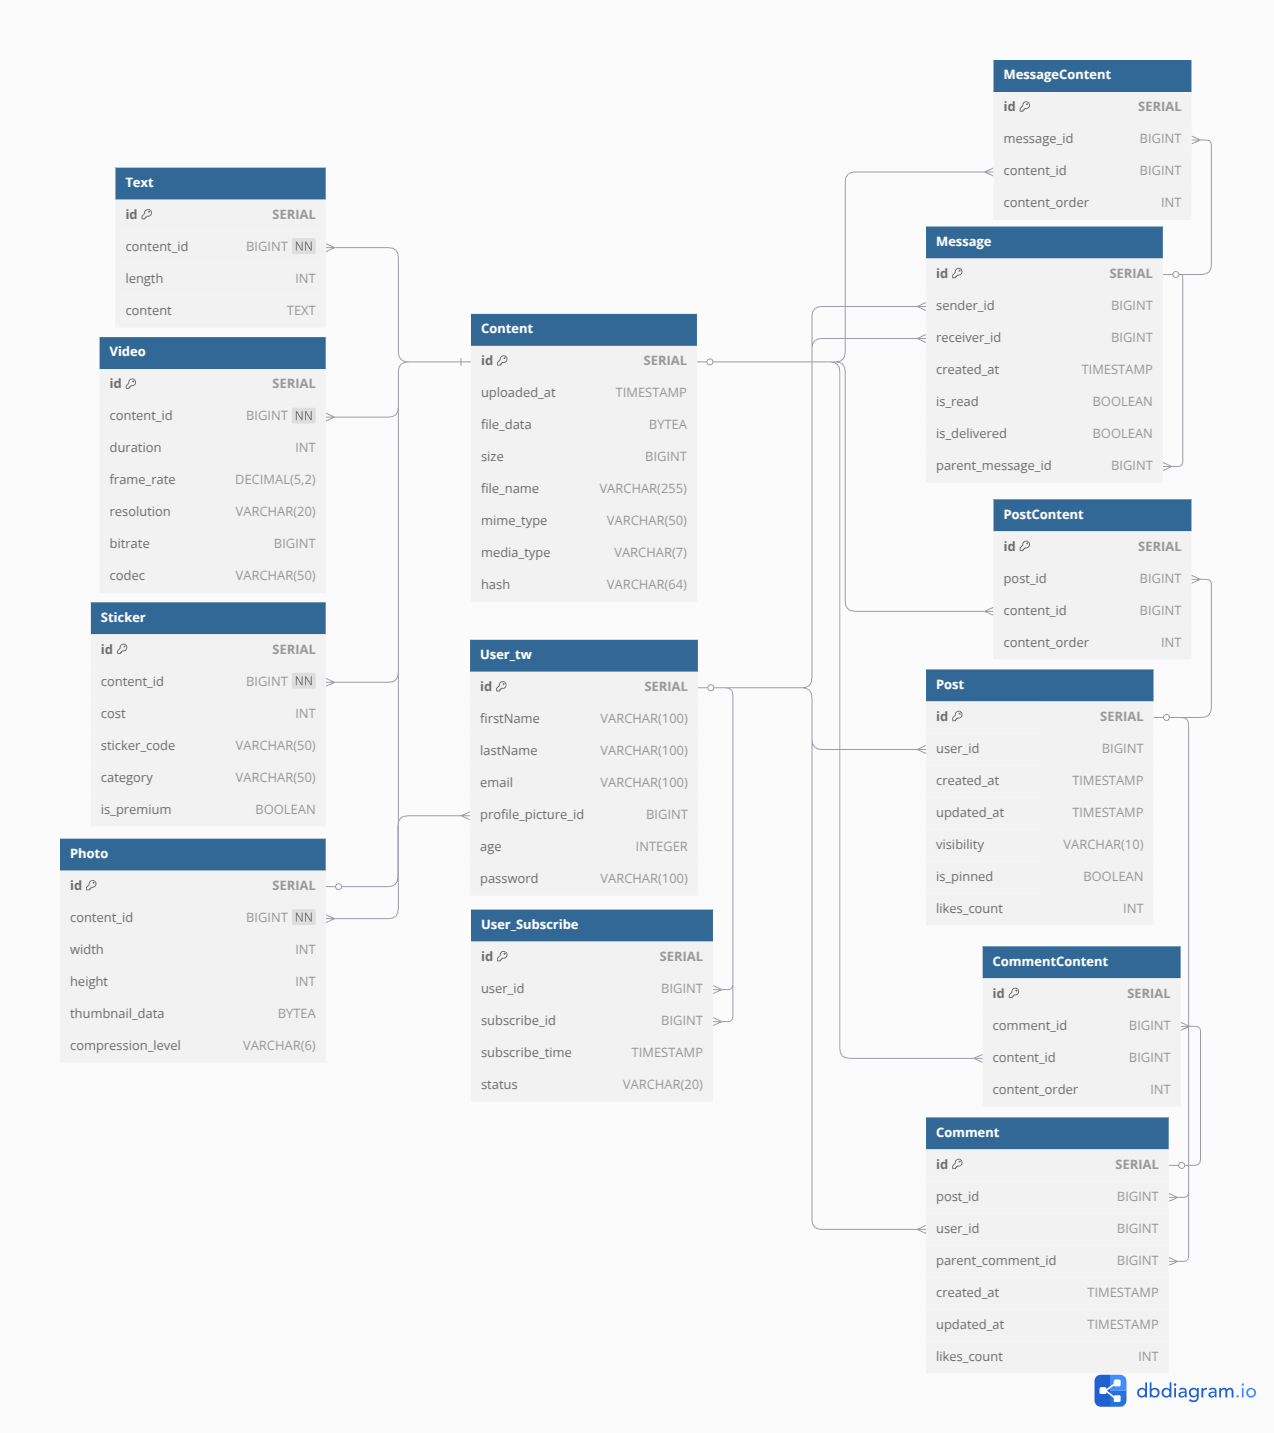
\includegraphics[width=0.8\textwidth]{postgres.png}
\end{center}

Примеры запросов:
\\ \\
Задача: Найти 10 самых популярных элементов контента (фото, видео, текст, стикеры) за последний месяц, 
основываясь на общем количестве лайков постов, в которых они использовались. 
Также, для каждого элемента контента, вернуть имена и email создателей этих постов.

Сложность: Требует объединения множества таблиц (Content, PostContent, Post, User\_tw) и агрегации данных. 
Сложно масштабировать при увеличении объема данных.

\begin{lstlisting}[caption={TOP10}, label={lst:example}]
    EXPLAIN ANALYZE
    SELECT
        c.id AS content_id,
        c.media_type,
        c.file_name,
        SUM(p.likes_count) AS total_likes,
        STRING_AGG(DISTINCT u.firstName || ' ' || u.lastName, ', ') AS creator_names,
        STRING_AGG(DISTINCT u.email, ', ') AS creator_emails
    FROM
        Content c
    JOIN
        PostContent pc ON c.id = pc.content_id
    JOIN
        Post p ON pc.post_id = p.id
    JOIN
        User_tw u ON p.user_id = u.id
    WHERE
        p.created_at >= NOW() - INTERVAL '1 month'
    GROUP BY
        c.id, c.media_type, c.file_name
    ORDER BY
        total_likes DESC
    LIMIT 10;
\end{lstlisting}

\begin{lstlisting}[caption={explain analyze without indexes}, label={lst:example}]
    Planning Time: 0.232 ms
    Execution Time: 206.047 ms
\end{lstlisting}
\begin{lstlisting}[caption={explain analyze with indexes}, label={lst:example}]
    Planning Time: 0.613 ms
    Execution Time: 191.192 ms
\end{lstlisting}

Задача: Для заданного пользователя (например, с user\_id = 123), найти 5 наиболее подходящих элементов контента,
которые он еще не видел, основываясь на следующих критериях:
У контента есть лайки.
Контент от пользователей, на которых он подписан.
В данном случае, будем считать, что "похожий" контент - это контент того же media\_type.

Сложность: Требует объединения таблиц подписок, постов, контента и пользователей, 
а также логики для фильтрации просмотренного контента.
\begin{lstlisting}[caption={recommend}, label={lst:example}]
    EXPLAIN ANALYZE
    WITH user_likes AS (
        SELECT DISTINCT c.media_type
        FROM Post p
        JOIN PostContent pc ON p.id = pc.post_id
        JOIN Content c ON pc.content_id = c.id
        WHERE p.user_id = 123 AND p.likes_count > 0 
    ),
    subscribed_users_content AS (
        SELECT c.id AS content_id, c.media_type, p.created_at
        FROM User_Subscribe us
        JOIN Post p ON us.subscribe_id = p.user_id
        JOIN PostContent pc ON p.id = pc.post_id
        JOIN Content c ON pc.content_id = c.id
        WHERE us.user_id = 123 AND us.status = 'approved'
    ),
    similar_content AS (
        SELECT c.id AS content_id, c.media_type, p.created_at
        FROM Post p
        JOIN PostContent pc ON p.id = pc.post_id
        JOIN Content c ON pc.content_id = c.id
        JOIN user_likes ul ON c.media_type = ul.media_type
        WHERE p.user_id <> 123 
    )
    SELECT content_id, media_type
    FROM (
        SELECT content_id, media_type, created_at FROM subscribed_users_content
        UNION ALL
        SELECT content_id, media_type, created_at FROM similar_content
    ) AS combined_content
    WHERE content_id NOT IN (SELECT content_id FROM PostContent WHERE post_id IN (SELECT id FROM Post WHERE user_id = 123)) 
    ORDER BY created_at DESC
    LIMIT 5;
\end{lstlisting}
\begin{lstlisting}[caption={explain analyze without indexes}, label={lst:example}]
    Planning Time: 0.459 ms
    Execution Time: 79.735 ms
\end{lstlisting}
\begin{lstlisting}[caption={explain analyze with indexes}, label={lst:example}]
    Planning Time: 0.964 ms
    Execution Time: 55.243 ms
\end{lstlisting}

Задача: Найти всех пользователей, которые подписаны друг на друга (A подписан на B, и B подписан на A).

Сложность: Требует self-join и проверки условия взаимности.
\begin{lstlisting}[caption={subs}, label={lst:example}]
    EXPLAIN ANALYZE
    SELECT
        us1.user_id AS user1_id,
        us2.user_id AS user2_id
    FROM
        User_Subscribe us1
    JOIN
        User_Subscribe us2 ON us1.user_id = us2.subscribe_id AND us1.subscribe_id = us2.user_id
    WHERE
        us1.user_id < us2.user_id  
        AND us1.status = 'approved'
        AND us2.status = 'approved';
\end{lstlisting}
\begin{lstlisting}[caption={explain analyze without indexes}, label={lst:example}]
    Planning Time: 0.099 ms
    Execution Time: 22.437 ms
\end{lstlisting}
\begin{lstlisting}[caption={explain analyze with indexes}, label={lst:example}]
    Planning Time: 0.267 ms
    Execution Time: 16.065 ms
\end{lstlisting}

\section{MongoDB}

Задача: Найти 10 самых популярных элементов контента (фото, видео, текст, стикеры) за последний месяц, 
основываясь на общем количестве лайков постов, в которых они использовались. 
Также, для каждого элемента контента, вернуть имена и email создателей этих постов.
\begin{lstlisting}[caption={analyze without indexes}, label={lst:example}]
    Query 1 (Top 10 popular): 0s 53.351318ms
\end{lstlisting}
\begin{lstlisting}[caption={analyze with indexes}, label={lst:example}]
    
\end{lstlisting}

Задача: Для заданного пользователя (например, с user\_id = 123), найти 5 наиболее подходящих элементов контента,
которые он еще не видел, основываясь на следующих критериях:
У контента есть лайки.
Контент от пользователей, на которых он подписан.
В данном случае, будем считать, что "похожий" контент - это контент того же media\_type.
\begin{lstlisting}[caption={analyze without indexes}, label={lst:example}]
    Query 2 (Recommendations): 0s 261.533013ms
\end{lstlisting}
\begin{lstlisting}[caption={analyze with indexes}, label={lst:example}]
    
\end{lstlisting}

Задача: Найти всех пользователей, которые подписаны друг на друга (A подписан на B, и B подписан на A).
\begin{lstlisting}[caption={analyze without indexes}, label={lst:example}]
    Query 3 (Mutual subs): 3s 69.803046ms\end{lstlisting}
\begin{lstlisting}[caption={analyze with indexes}, label={lst:example}]
    
\end{lstlisting}



\end{document}


















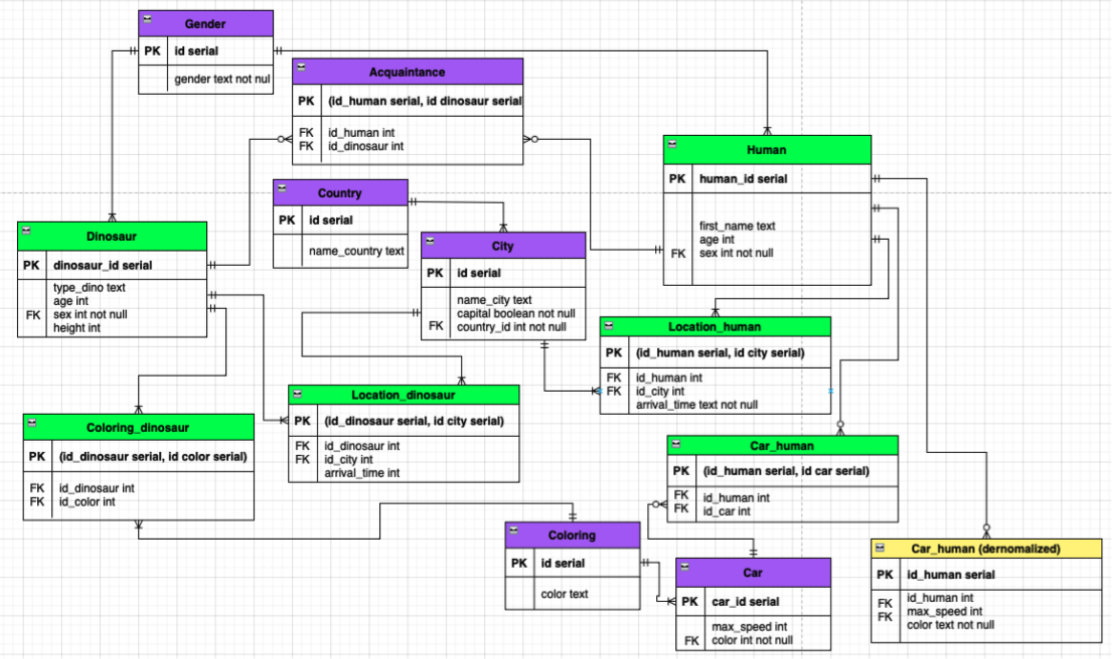
\includegraphics[width=.9\textwidth]{123}

\begin{lstlisting}[caption={kitty}, label={lst:example}]

\end{lstlisting}